\documentclass[a4paper,landscape,10pt]{article}
\usepackage[left=1.0cm,right=1.0cm,top=1.0cm,bottom=1.2cm]{geometry}
\usepackage{longtable}
\usepackage{array}
\usepackage{xcolor}
\usepackage{helvet}
\usepackage{colortbl}
\usepackage{fancyhdr}
\usepackage[hidelinks]{hyperref}
\usepackage{graphicx}

\renewcommand{\familydefault}{\sfdefault}
\pagestyle{fancy}
\fancyhf{}
\rhead{\footnotesize GEMASTIK XIX 2026 -- Divisi Pengembangan Perangkat Lunak -- Tim Three Achilles (TRPL SV UGM)}
\lhead{\footnotesize Storyboard Produksi Video Karya Akhir 100\%: Verifin}
\rfoot{\footnotesize Halaman \thepage}

\setlength{\parindent}{0pt}
\renewcommand{\arraystretch}{1.25}
\setlength{\tabcolsep}{3.5pt}

% Custom column types with clean wrapping
\newcolumntype{C}[1]{>{\centering\arraybackslash}p{#1}}
\newcolumntype{L}[1]{>{\raggedright\arraybackslash}p{#1}}

\begin{document}

% Metadata Header
\begin{minipage}[t]{0.70\textwidth}
\textbf{GEMASTIK XIX 2026 -- Divisi PPL} \\
\begin{tabular}{@{}ll@{}}
\textbf{Talent} & : Rama (Fresh Grad), Dosen TRPL SV UGM, Tim Three Achilles (Hafidz, Matthew, Akmal), Teman 1 \& 2 \\
\textbf{Lokasi Shooting} & : Kafe Jogja, Ruang Dosen TILC SV UGM, Lab Rekayasa Perangkat Lunak SV UGM, Selasar SV UGM \\
\textbf{Properti} & : Smartphone (chat WA scam), Workstation Dual-Screen, Berkas Cetak BUMN, Jas Almamater UGM \\
\end{tabular}
\end{minipage}
\hfill
\begin{minipage}[t]{0.28\textwidth}
\raggedleft
\textbf{Total Durasi Target}: 10:00 (595 Detik) \\
\textbf{Format Video}: MP4 1080p / 720p 60fps \\
\textbf{Status Karya}: 100\% Live Deployment \\
\end{minipage}

\vspace{0.25cm}
\begin{center}
{\Large \textbf{STORYBOARD ``VERIFIN: GARDA TALENTA DIGITAL''}} \\
\vspace{0.08cm}
{\small \textbf{Sistem Deteksi Lowongan Kerja Palsu Berbasis AI \& OSINT -- Karya Akhir 100\%}}
\end{center}
\vspace{0.15cm}

\begin{longtable}{|C{1.2cm}|C{1.2cm}|L{2.0cm}|L{1.8cm}|L{1.8cm}|L{4.0cm}|L{8.2cm}|C{1.1cm}|L{4.0cm}|}
\hline
\rowcolor{gray!20}
\textbf{Scene} & \textbf{Int/Eks} & \textbf{Jenis Shoot} & \textbf{Camera Move} & \textbf{Audio} & \textbf{Visual} & \textbf{Deskripsi} & \textbf{Durasi} & \textbf{Keterangan} \\
\hline
\endfirsthead

\hline
\rowcolor{gray!20}
\textbf{Scene} & \textbf{Int/Eks} & \textbf{Jenis Shoot} & \textbf{Camera Move} & \textbf{Audio} & \textbf{Visual} & \textbf{Deskripsi} & \textbf{Durasi} & \textbf{Keterangan} \\
\hline
\endhead

\multicolumn{9}{|c|}{\cellcolor{gray!15}\textbf{bumper}} \\
\hline
Bumper & - & Full Screen & Still & SFX Bumper & Logo Kemendikbudristek, Puspresnas, GEMASTIK XIX \& UGM & Animasi bumper pembuka resmi kompetisi GEMASTIK XIX 2026 dan Universitas Gadjah Mada & 5 dtk & Fade in to scene 1 \\
\hline

\multicolumn{9}{|c|}{\cellcolor{gray!10}\textbf{BABAK I: THE REALITY \& THE DILEMMA (00:00 -- 02:00)}} \\
\hline
1 & Eks & Wide & Pan right & Ambience jalan \& kafe & Fasad depan coffee shop Jogja, kendaraan terparkir & Suasana sore di kafe tempat berkumpulnya reuni alumni muda TRPL SV UGM & 6 dtk & Establishing shot pembuka suasana \\
\hline
2 & Int & Medium & Still & Ambience kafe, tawa & Meja kafe, cangkir kopi, 3 alumni muda duduk santai\par\vspace{3pt}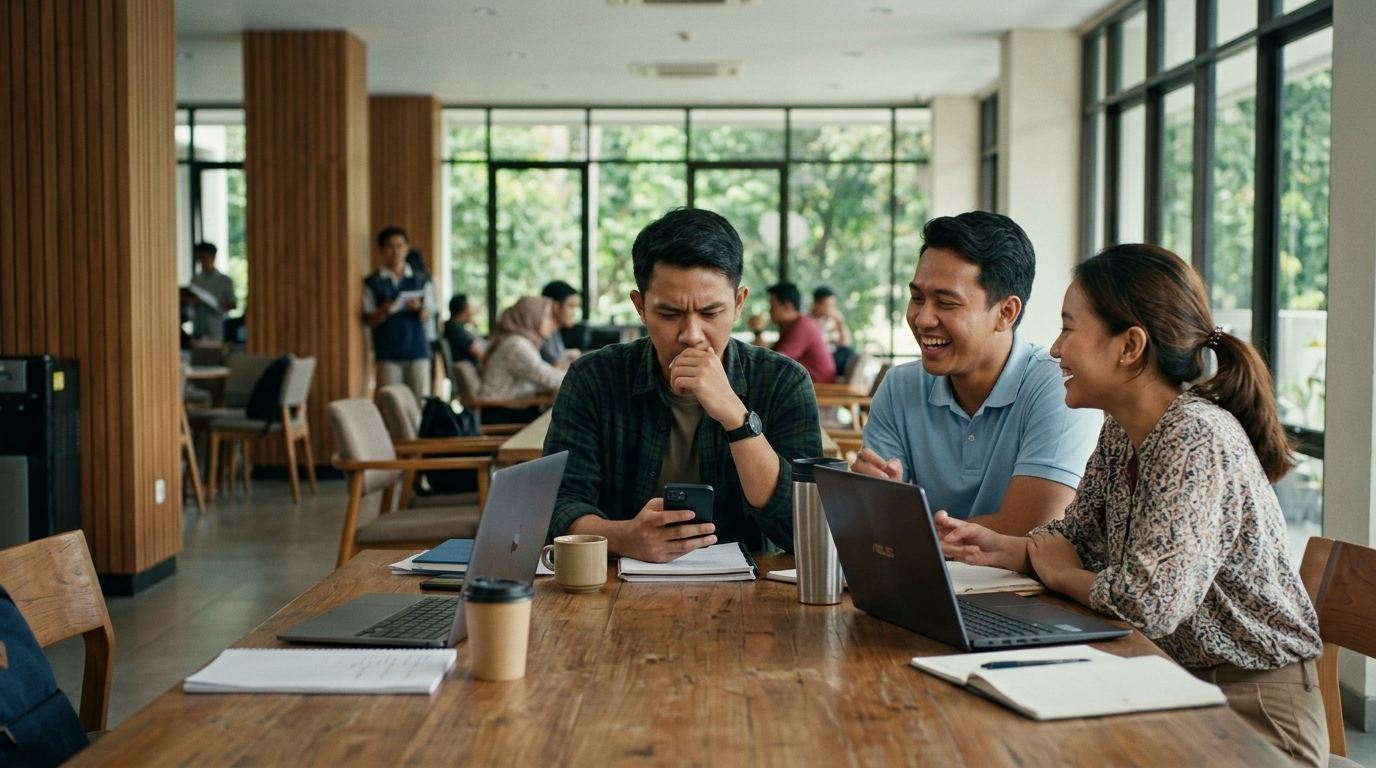
\includegraphics[width=\linewidth]{images/scene_2.jpg} & Teman 1 dan 2 seru mengobrolkan kantor baru, Rama duduk melamun memperhatikan ponselnya & 9 dtk & Shot dari depan meja \\
\hline
3 & Int & Over the Shoulder & Still & Ambience kafe & Layar smartphone Rama menampilkan chat WA asing & Kamera dari balik bahu menyorot tawaran Admin WFH gaji 15 juta tapi wajib transfer deposit seragam 500rb \& selfie KTP & 7 dtk & Focus pull dari bahu ke layar ponsel \\
\hline
4 & Int & Close Up & Slow push-in & Dialog Rama & Wajah Rama tampak gelisah dan lelah & \textbf{Rama}: ``Gue lagi overthinking parah bro... Ada panggilan Admin WFH gaji dua digit, tapi disuruh transfer uang registrasi 500 ribu dan minta selfie KTP.'' & 13 dtk & Shot ekspresi bimbang talent \\
\hline
5 & Int & Medium & Still & Dialog Teman 1 \& 2 & Teman 1 \& 2 menanggapi dengan kaget & \textbf{Teman 1}: ``Waduh, bahaya itu Ram! Jangan asal transfer!'' \newline \textbf{Teman 2}: ``Modus begitu marak banget, ujungnya KTP lu disalahgunakan buat pinjol ilegal.'' & 12 dtk & Two-shot reaksi teman reuni \\
\hline
6 & Int & Close Up & Still & Dialog Rama & Rama menatap cangkirnya lalu melihat temannya & \textbf{Rama}: ``Masalahnya gue udah 4 bulan wisuda belum dapet kerja... Takut ini tipuan, tapi takut nolak kalau ternyata beneran rezeki. Kita orang awam susah banget bedain PT fiktif sama yang asli sekarang.'' & 18 dtk & Freeze frame di wajah Rama di akhir dialog \\
\hline
7 & - & Motion Graphic & Zoom in / Pan & SFX Glitch \& Whoosh & Chat WA Rama melayang keluar layar HP menjadi 3D HUD card & Kotak scanner merah berkedip mengunci kata kunci:\newline $\bullet$ [UNREALISTIC SALARY]\newline $\bullet$ [UPFRONT PAYMENT TRAP]\newline $\bullet$ [IDENTITY THEFT RISK] & 8 dtk & Motion HUD floating UI overlay \\
\hline
8 & - & Motion Graphic & Dynamic Orbit & SFX Ticker \& Synth & Peta 3D Indonesia dengan titik hotspot merah menyala & Animasi counter ticker data darurat:\newline $\bullet$ 7,28 Juta Pengangguran (BPS)\newline $\bullet$ 49\% Korban Scam Modus Loker (GASA)\newline $\bullet$ Kerugian Rp49 Triliun\newline $\bullet$ 3.300+ Korban TPPO Siber (Kemenlu) & 20 dtk & Kinetic typography \& infografis 3D \\
\hline
9 & - & Motion Graphic & Center Reveal & SFX Hit Impact & Logo VERIFIN muncul dengan partikel neon bercahaya & Title resmi:\newline \textbf{VERIFIN: Deteksi Lowongan Kerja Palsu Berbasis AI \& OSINT}\newline Three Achilles -- TRPL SV UGM & 10 dtk & Match cut ke pintu ruang dosen \\
\hline

\multicolumn{9}{|c|}{\cellcolor{gray!10}\textbf{BABAK II: THE BRIDGE \& READY-TO-USE PLATFORM (02:00 -- 03:15)}} \\
\hline
10 & Int & Medium & Track in & Ambience tenang & Pintu ruang dosen dibuka dari luar & Rama melangkah masuk ke ruang dosen Gedung TILC SV UGM, menyapa dosen & 6 dtk & Shot dari dalam ruangan dosen \\
\hline
11 & Int & Two Shot & Still & Dialog Rama \& Dosen & Dosen dan Rama duduk berhadapan di meja kerja & \textbf{Rama}: ``Saya bingung Pak cara verifikasi loker yang aman... Kalau cuma modal feeling sering bias dan takut kena tipu.'' & 14 dtk & Shot formal berwibawa \\
\hline
12 & Int & Medium Close Up & Still & Dialog Dosen & Dosen tersenyum menenangkan dan memberi solusi\par\vspace{3pt}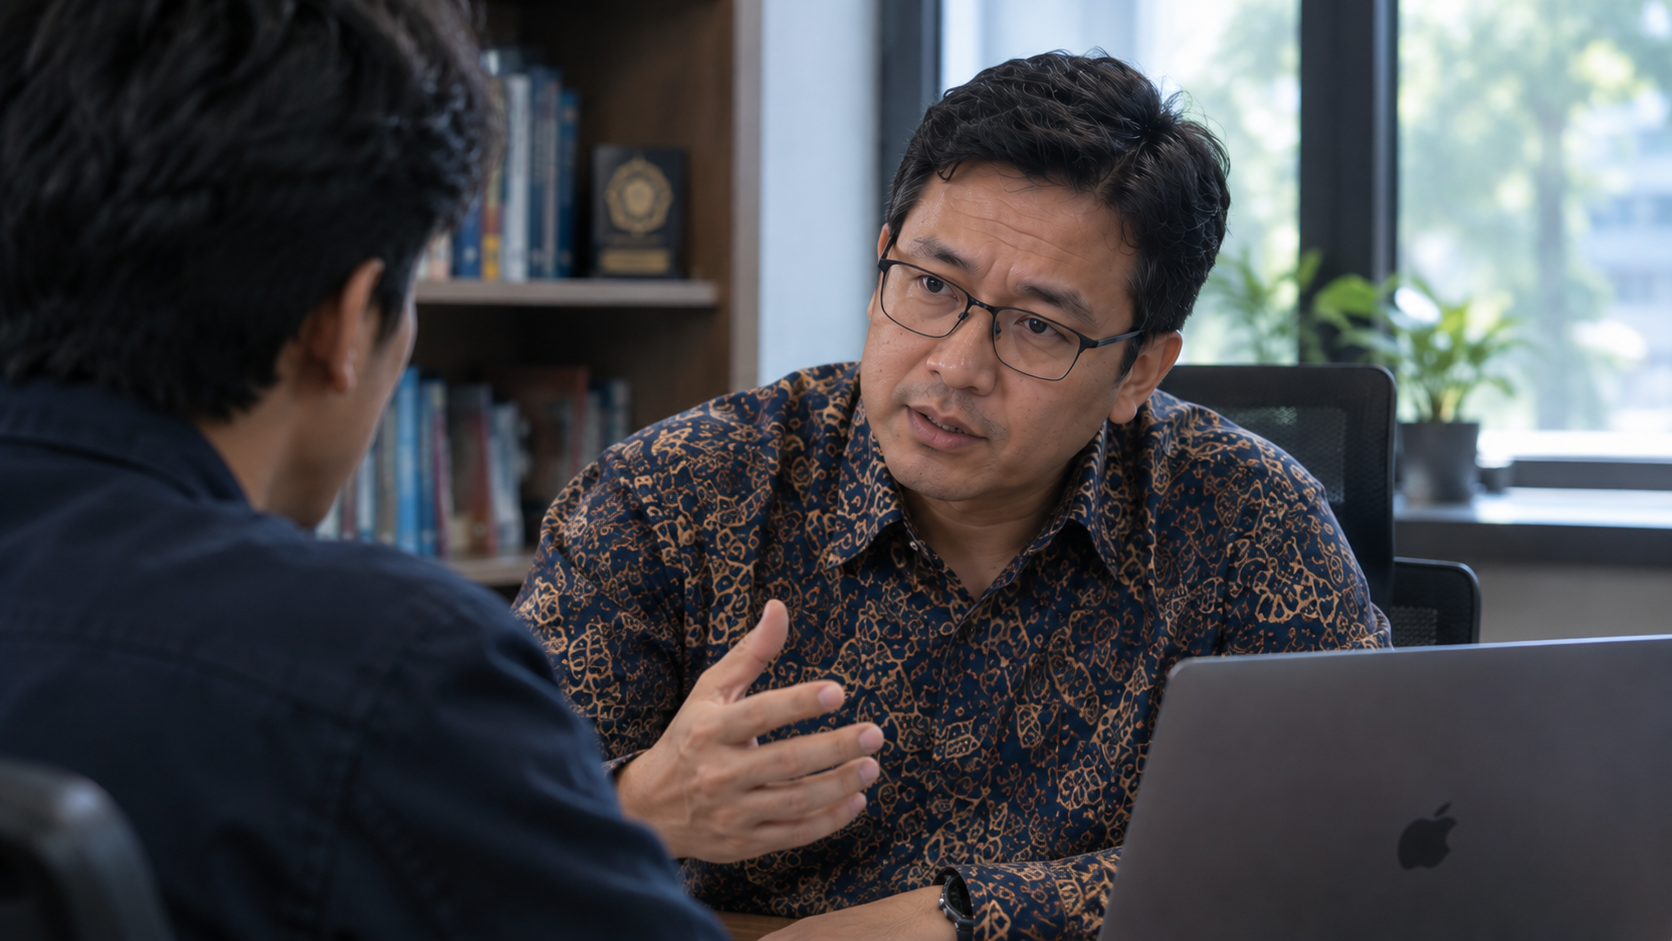
\includegraphics[width=\linewidth]{images/scene_12.png} & \textbf{Dosen}: ``Keputusan kamu tepat untuk tidak buru-buru transfer, Rama. Justru di kampus kita, rekan-rekan TRPL SV UGM sudah merilis platform khusus untuk menangani ini: \textbf{Verifin}. Sistemnya sudah live, siap digunakan publik, menggabungkan AI dan OSINT. Ayo kita ke lab, kamu bisa langsung buka dan pakai platformnya sekarang juga.'' & 25 dtk & Shot dari samping meja dosen \\
\hline
13 & Eks & Medium & Tracking walk & Ambience selasar & Dosen dan Rama berjalan bersama di selasar TILC & Dosen dan Rama berjalan menuju Laboratorium Rekayasa Perangkat Lunak SV UGM & 8 dtk & Dolly samping mengikuti langkah kaki talent \\
\hline
14 & Int & Wide & Pan left & Ambience lab PC & Lab Software Engineering TRPL SV UGM & Workstation monitor dual-screen menampilkan live dashboard Verifin. Hafidz, Matthew, dan Akmal sedang standby & 9 dtk & Establishing ruang laboratorium \\
\hline
15 & Int & Medium & Still & Dialog Tim & Hafidz, Matthew, dan Akmal menyapa Dosen \& Rama & \textbf{Dosen}: ``Ini Rama alumni kita mau cek tawarannya.''\newline \textbf{Hafidz}: ``Halo Mas Rama! Pas banget, Verifin memang sudah kami rilis dan aktif beroperasi untuk melayani pencari kerja secara real-time. Mas bisa langsung buka web kami sekarang juga.'' & 18 dtk & Group shot tim menyambut Rama \\
\hline
16 & Int & Over the Shoulder & Still & Dialog Rama \& Matthew & Rama duduk di depan workstation, Matthew mendampingi & \textbf{Matthew}: ``Platform kami sudah terintegrasi menyeluruh dari OSINT sampai graf jaringan penipuan. Mas Rama bawa berkas lokernya? Langsung kita input ke platformnya!''\newline \textbf{Rama}: ``Gue bawa dua: yang satu surat panggilan resmi BUMN, satu lagi poster loker toko lokal tapi pakai Gmail.'' & 18 dtk & Kamera fokus ke Rama yang mengeluarkan berkas \\
\hline

\multicolumn{9}{|c|}{\cellcolor{gray!10}\textbf{BABAK III: THE BATTLE OF EDGE CASES -- LIVE DEMO 100\% (03:15 -- 06:45)}} \\
\hline
17 & Int & Screen Capture & Still & SFX Klik mouse & Layar monitor menampilkan homepage web live Verifin (Next.js 16) & Akmal mengarahkan Rama memilih kanal Input Teks \& Link. Rama meng-copy isi surat panggilan wawancara BUMN tiruan & 10 dtk & Screen recording jernih 1080p \\
\hline
18 & Int & Close Up & Still & Dialog Rama & Rama menunjukkan klausul di kertas berkas & \textbf{Rama}: ``Liat nih bro, kop suratnya resmi BUMN Semen Indonesia, ada stempelnya. Tapi di halaman 2 wajib pesan tiket pesawat via biro travel rekanan (PT Global Travelindo) dan nanti di-reimburse.'' & 15 dtk & Shot kertas surat dan wajah heran Rama \\
\hline
19 & - & Screen Capture & Slow zoom & SFX Processing & Link recruitment-semenindonesia.xyz di-paste \& tombol ``Analisis Sekarang'' ditekan & Progress bar multi-tahap berjalan interaktif:\newline [1/5 NER Extraction] $\rightarrow$ [2/5 NLP] $\rightarrow$ [3/5 OSINT Parallel] & 12 dtk & Animasi HUD processing bar \\
\hline
20 & - & Screen Capture & Still & SFX Alert Horn & Dashboard Hasil: Trust Score Gauge berputar ke 94/100, Badge Merah: BAHAYA\par\vspace{3pt}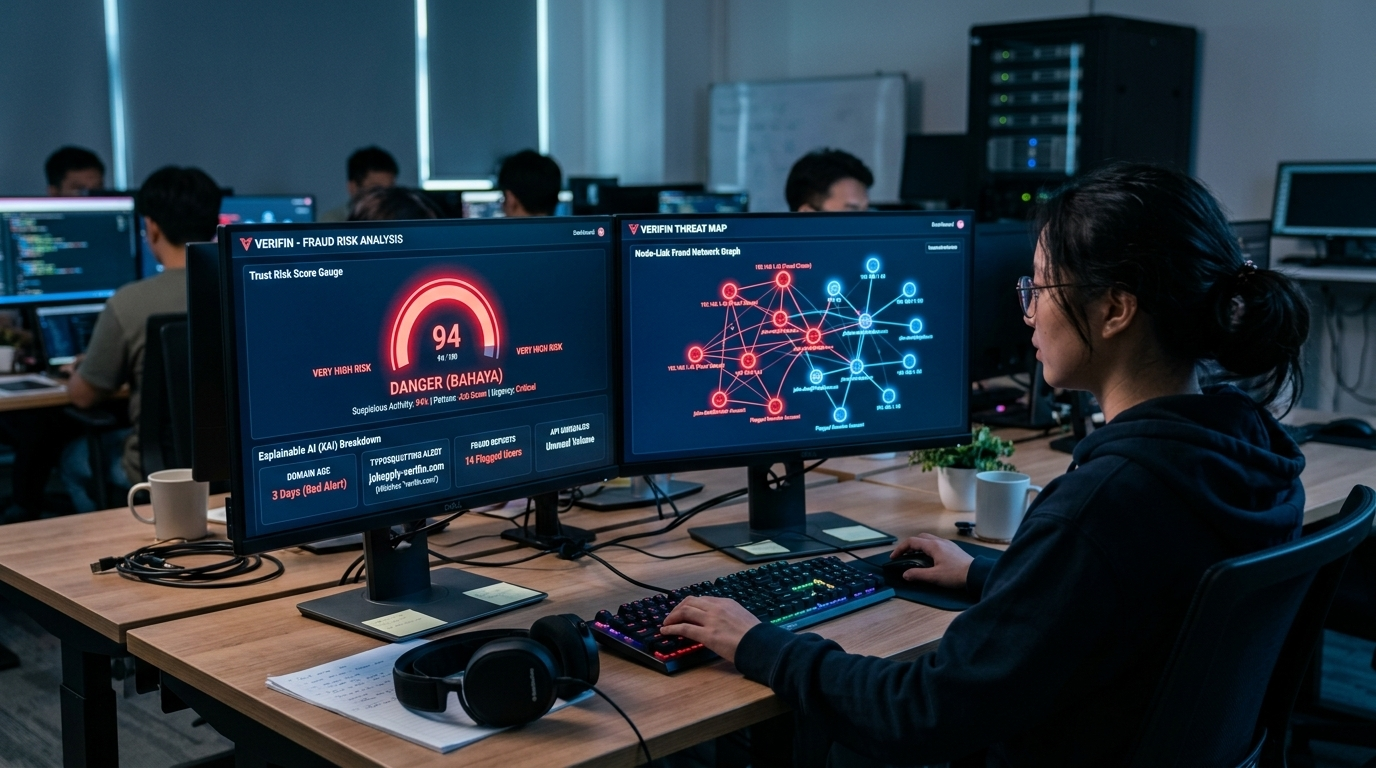
\includegraphics[width=\linewidth]{images/scene_20.jpg} & Layar split-screen: Hasil Verifin di kiri, wajah kaget Rama \& Matthew di kanan.\newline Kartu XAI merah:\newline $\bullet$ Domain Age: 5 Hari (Penalti +30)\newline $\bullet$ Typosquatting .xyz vs Resmi .co.id\newline $\bullet$ Biro Travel: 14 Laporan Fraud di Kredibel.id (Penalti +35) & 20 dtk & Worst-Case FAKE terbongkar tuntas \\
\hline
21 & Int & Medium & Still & Dialog Matthew \& Rama & Matthew menunjuk ke layar monitor, Rama tertegun\par\vspace{3pt}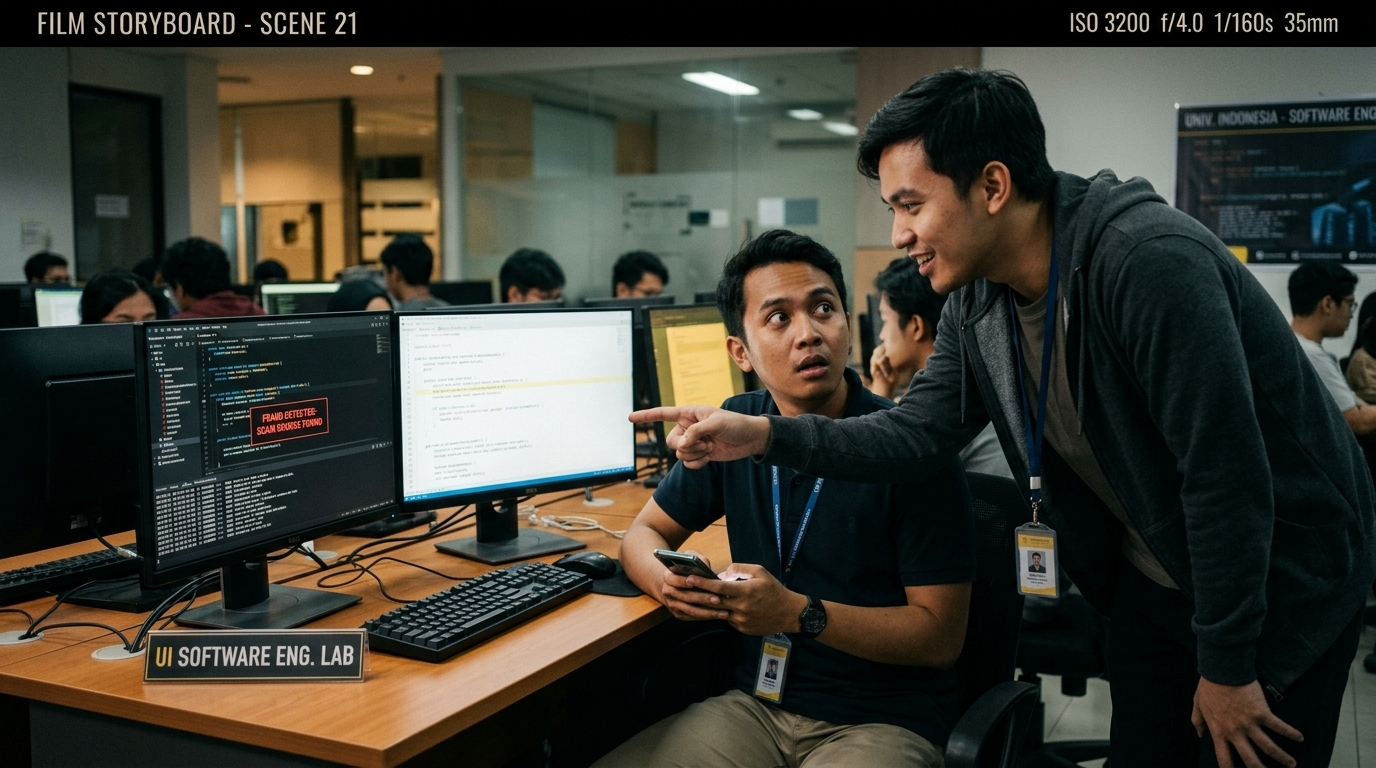
\includegraphics[width=\linewidth]{images/scene_21.jpg} & \textbf{Matthew}: ``Bisa dilihat Mas Rama, suratnya rapi, tapi mesin OSINT Verifin membongkar bahwa domain ini baru dibuat 5 hari lalu! Dan nomor biro travelnya sudah punya 14 laporan penipuan tiket di Kredibel!''\newline \textbf{Rama}: ``Gila! Kalau gue modal percaya kop surat doang, duit gue pasti ludes jutaan buat tiket fiktif!'' & 20 dtk & Reaksi emosional talent \\
\hline
22 & Int & Screen Capture & Pan down & SFX Klik tab & Tab Fraud Network Graph dibuka & Layar menampilkan graf interaktif (React Flow + D3.js). Node nomor HP penipu menyala merah dan terhubung ke 3 node kasus PT fiktif lainnya di database & 15 dtk & Pembuktian intelijen graf sindikat \\
\hline
23 & Int & Medium & Still & Dialog Hafidz & Hafidz menjelaskan basis data graf & \textbf{Hafidz}: ``Karena Verifin sudah beroperasi aktif, database kami sudah memetakan ratusan fingerprint penipuan. Nomor ini terbukti terkoneksi ke sindikat penipuan yang sama di beberapa kota.'' & 14 dtk & Shot Hafidz menjelaskan data \\
\hline
24 & Int & Close Up & Still & Dialog Rama \& Akmal & Rama menunjukkan poster di HP: The Biker Shop Jogja & \textbf{Rama}: ``Nah kalau yang kedua ini gimana? Poster loker toko sepeda motor lokal, tapi daftarnya lewat Google Form dan emailnya cuma pakai Gmail gratisan (hrdthebikershop@gmail.com). Ini jangan-jangan scam juga?'' & 17 dtk & Worst-Case VALID dimulai \\
\hline
25 & Int & Screen Capture & Still & SFX Typing & Teks loker The Biker Shop diinput ke Verifin & Akmal memasukkan teks loker The Biker Shop ke kanal input Verifin dan menekan tombol analisis & 9 dtk & Screen recording input teks \\
\hline
26 & - & Screen Capture & Still & SFX Success Ping & Dashboard Hasil muncul: Skor 15/100, Badge Hijau: AMAN (Tervalidasi) & Tampil callout kartu XAI warna hijau lembut:\newline $\bullet$ Alamat Fisik Valid: Jl. Parangtritis No. 38 (OpenStreetMap)\newline $\bullet$ Medsos Aktif: IG @thebikershop.jogja (1.6K Followers)\newline $\bullet$ Aturan Perilaku: Tanpa Biaya (Penalti 0) & 20 dtk & Anti-False Positive terbukti nyata \\
\hline
27 & Int & Medium & Still & Dialog Akmal \& Hafidz & Akmal dan Hafidz menjelaskan di depan monitor & \textbf{Akmal}: ``Inilah keunggulan Verifin, Mas Rama. Sistem kami tidak sembarangan memvonis hanya karena email Gmail. Mesin OSINT memverifikasi bahwa toko fisiknya benar-benar nyata di Jalan Parangtritis Jogja, akun media sosialnya aktif berniaga, dan nomornya bersih dari riwayat kejahatan.''\newline \textbf{Hafidz}: ``Dengan fitur Anti-False Positive, bisnis UMKM lokal tetap terlindungi dan pencari kerja tidak kehilangan peluang kerja sah.'' & 25 dtk & Shot edukasi nilai inovasi sistem \\
\hline
28 & Int & Medium & Still & Dialog Rama & Rama tersenyum lega menatap layar & \textbf{Rama}: ``Wah, presisi banget sistemnya! Jadi gue tahu pasti kalau toko ini beneran aman buat gue lamar.'' & 8 dtk & Shot kepuasan pengguna \\
\hline
29 & Int & Screen Capture & Still & SFX Shutter & Halaman input OCR Gambar diuji & Matthew mengunggah poster gambar buram (VinFast Yogyakarta). PaddleOCR 2.8 mengekstrak teks otomatis $\rightarrow$ hasil keluar: WASPADA (Skor 48) karena memakai nomor perorangan tanpa web resmi dealer & 16 dtk & Demo kanal OCR 100\% \\
\hline
30 & Int & Screen Capture & Still & SFX Notifikasi & Tombol ``Laporkan ke Komunitas'' diklik oleh Rama & Form pelaporan terisi otomatis. Muncul badge notifikasi hijau: ``Laporan Terverifikasi \& Ditambahkan ke Community Feed Real-Time'' & 14 dtk & Demo fitur Community 100\% \\
\hline

\multicolumn{9}{|c|}{\cellcolor{gray!10}\textbf{BABAK IV: ENGINEERING EXCELLENCE \& ARCHITECTURE (06:45 -- 08:15)}} \\
\hline
31 & - & Motion Graphic 3D & Orbit 360$^\circ$ & SFX Whoosh \& Synth & Animasi tumpukan 5 lapisan kaca (Isometric Layer Stack) & Memvisualisasikan Arsitektur Pipeline 5-Layer:\newline $\bullet$ Layer 1: Hybrid NER (Regex + LLM)\newline $\bullet$ Layer 2: NLP Classifier (TF-IDF + LogReg)\newline $\bullet$ Layer 3: Parallel Async OSINT Engine\newline $\bullet$ Layer 4: LLM Evidence Synthesis\newline $\bullet$ Layer 5: Additive XAI Explainer ($S_{risiko} = S_{dasar} + \sum \phi_i$) & 30 dtk & Penjelasan arsitektur sistem \\
\hline
32 & Int & Medium & Still & Voiceover Hafidz & Hafidz berdiri di samping layar monitor arsitektur & \textbf{Hafidz (VO)}: ``Verifin tidak pernah memperlakukan AI sebagai 'black box'. Melalui Explainable AI di Layer 5, setiap poin risiko dihitung secara aditif dan transparan berdasarkan bukti fakta di lapangan, bukan sekadar gaya penulisan teks.'' & 20 dtk & Shot penjelasan teknis AI \\
\hline
33 & - & Motion Graphic & Pan right & SFX Typing & Terminal eksekusi automated testing \& chart evaluasi & $\bullet$ Automated test: pytest tests/ $\rightarrow$ 100\% PASSED (Coverage 91\%)\newline $\bullet$ Kurva evaluasi model ML: ROC-AUC mencapai 0,996 pada dataset EMSCAD\newline $\bullet$ Tampilan dashboard live container di Dokploy \& Cloudflare Tunnel & 24 dtk & Menjawab catatan juri soal software testing \\
\hline
34 & Int & Medium & Still & Dialog Akmal \& Matthew & Akmal \& Matthew bergantian menjelaskan proses SE & \textbf{Akmal}: ``Aplikasi dikembangkan menggunakan metode Agile Scrum dalam 4 sprint dengan arsitektur monorepo Next.js 16 dan FastAPI.''\newline \textbf{Matthew}: ``Pengujian end-to-end memastikan ketersediaan sistem di atas 95\% dengan waktu investigasi lengkap rata-rata di bawah 2 menit.'' & 18 dtk & Kredibilitas rekayasa software \\
\hline

\multicolumn{9}{|c|}{\cellcolor{gray!10}\textbf{BABAK V: RESOLUTION, IMPACT, \& CLOSING (08:15 -- 10:00)}} \\
\hline
35 & Int & Two Shot & Still & Dialog Dosen & Dosen menepuk bahu Rama dan tersenyum bangga\par\vspace{3pt}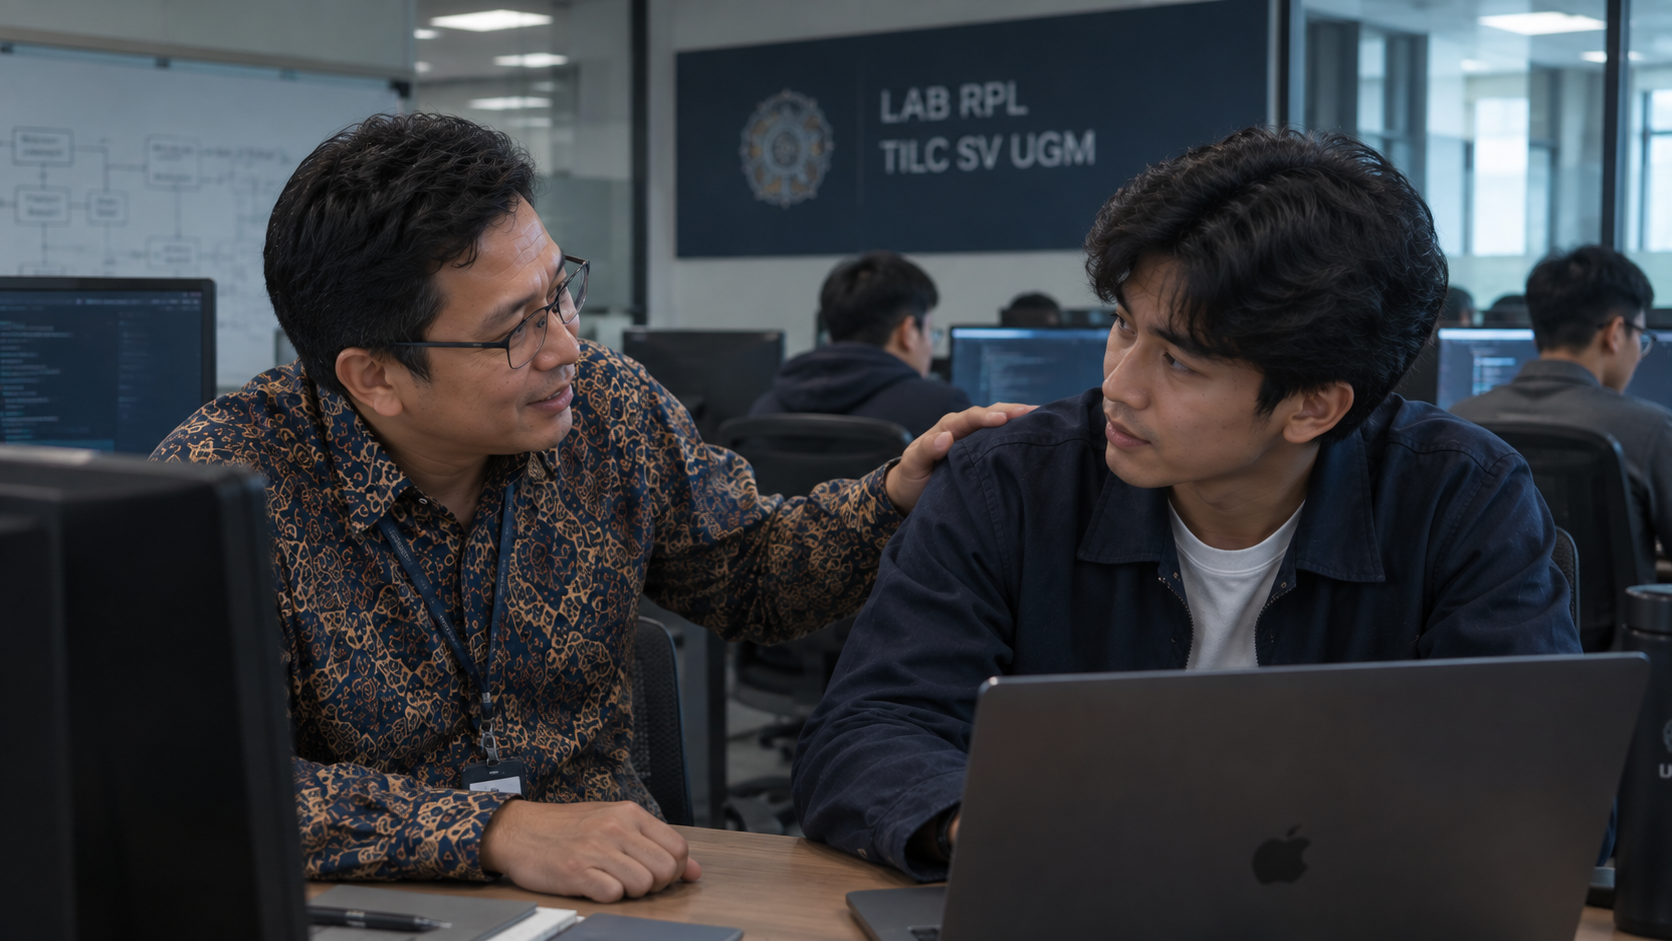
\includegraphics[width=\linewidth]{images/scene_35.png} & \textbf{Dosen}: ``Kerja keras yang luar biasa Three Achilles. Verifin membuktikan bahwa rekayasa perangkat lunak bukan hanya soal kecanggihan kode, tapi bagaimana teknologi hadir sebagai pelindung nyata bagi mereka yang sedang berjuang mencari nafkah.'' & 20 dtk & Apresiasi akademis \& etika \\
\hline
36 & Int & Close Up & Still & Dialog Rama & Rama tersenyum optimis sambil membuka web Verifin di HP & \textbf{Rama}: ``Terima kasih banyak Pak Ganjar dan tim Verifin! Rasanya bener-bener plong. Sekarang gue nggak was-was lagi, tiap ada loker masuk tinggal buka Verifin di HP buat cek keasliannya.'' & 15 dtk & Resolusi masalah karakter \\
\hline
37 & Eks & Medium Tracking & Dolly mundur & Music Up (Heroic) & Hafidz, Matthew, Akmal, dan Dosen berdiri di selasar SV UGM\par\vspace{3pt}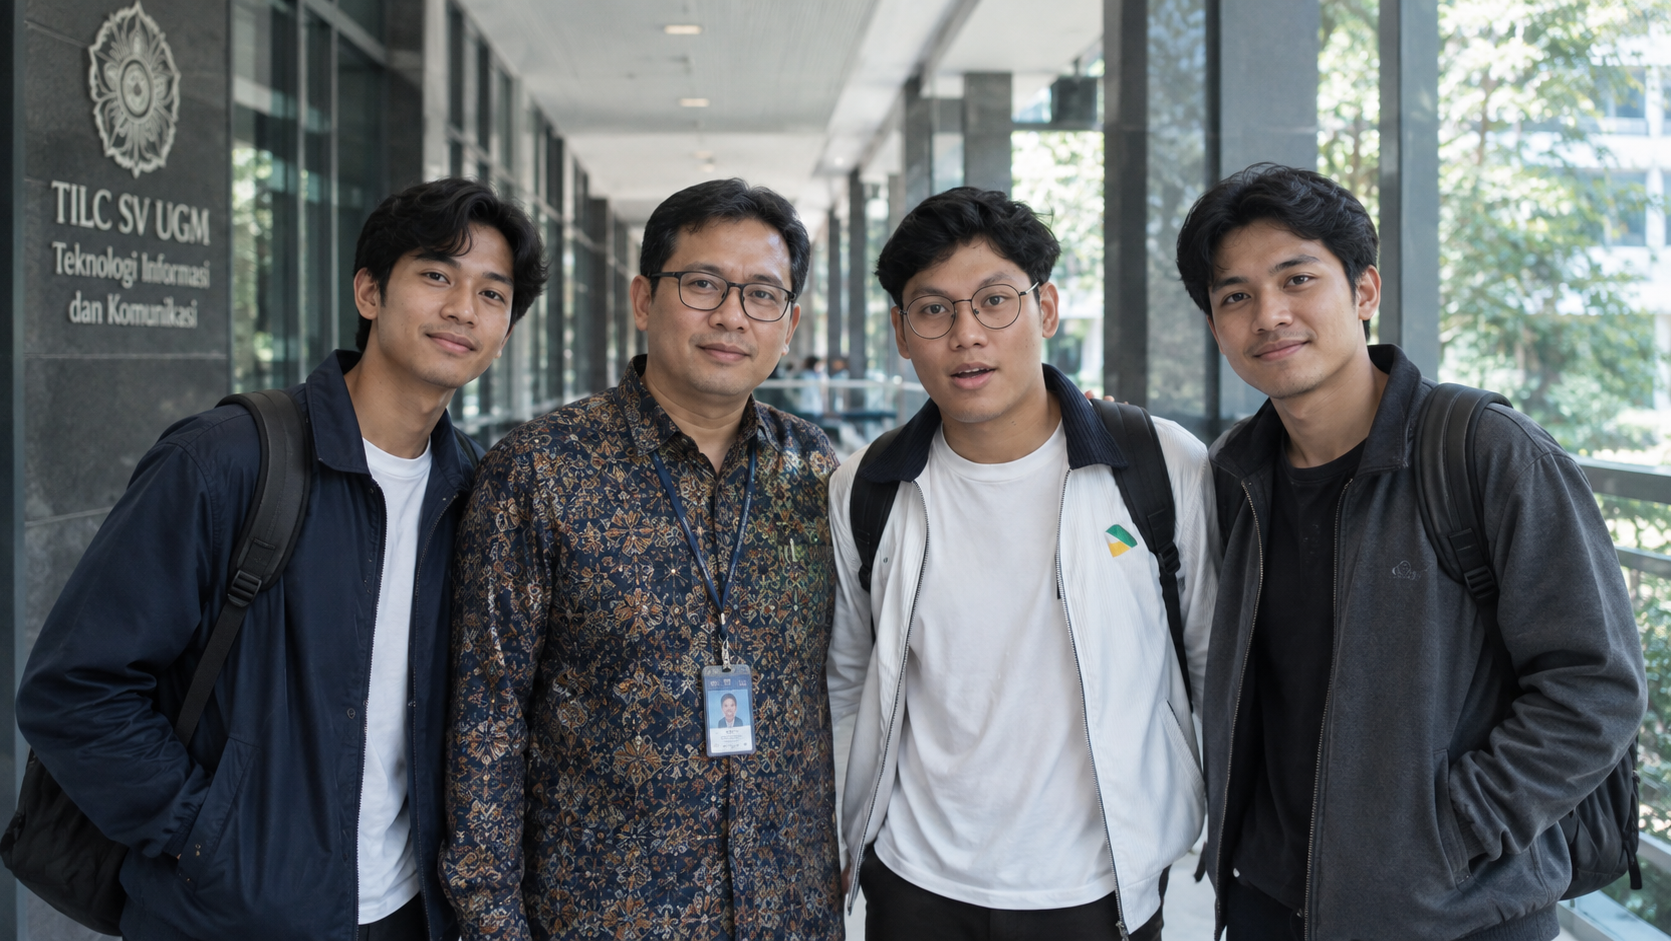
\includegraphics[width=\linewidth]{images/scene_37.png} & Seluruh tim mengenakan jas almamater UGM, melangkah mantap ke depan kamera di bawah sinar matahari hangat & 12 dtk & Visual sinematik klimaks \\
\hline
38 & Eks & Medium & Still & Orasi Penutup Tim & Kamera menyorot wajah anggota tim secara bergantian & \textbf{Hafidz}: ``Bagi jutaan pemuda Indonesia, lowongan kerja adalah gerbang masa depan, bukan perangkap keputusasaan.''\newline \textbf{Matthew}: ``Verifin kini telah hadir dan siap digunakan oleh seluruh masyarakat Indonesia.''\newline \textbf{Akmal}: ``Sebuah karya rekayasa perangkat lunak dari Sekolah Vokasi UGM untuk Indonesia yang aman dan berdaya.''\newline \textbf{Semua Bersama}: ``Kami Tim Three Achilles, siap mengawal talenta bangsa di GEMASTIK XIX 2026!'' & 35 dtk & Orasi penutup menggelegar \\
\hline

\multicolumn{9}{|c|}{\cellcolor{gray!15}\textbf{bumper}} \\
\hline
Bumper Outro & - & Full Screen & Still & SFX Ding \& Music Fade & Background Dark Slate Elegan & $\bullet$ Logo GEMASTIK XIX 2026 \& Logo Universitas Gadjah Mada\newline $\bullet$ Kartu QR Code \& URL Live App: verifin.app\newline $\bullet$ Badge Emas: PLATFORM LIVE \& SIAP DIGUNAKAN 100\%\newline $\bullet$ Credit Title: Tim Three Achilles -- D4 TRPL SV UGM 2026 & 18 dtk & Outro penutup video resmi \\
\hline

\end{longtable}

\end{document}
